\documentclass[UTF8,12pt,fontset=fandol]{ctexart}
\usepackage[a4paper,margin=27mm]{geometry}
\usepackage{amsmath,amssymb,amsthm,graphicx,booktabs}
\usepackage[backend=biber,style=numeric]{biblatex}
\addbibresource{references.bib}
\usepackage[colorlinks=true,linkcolor=blue,citecolor=blue]{hyperref}
\newcommand{\R}{\mathbb{R}}
\newtheorem{definition}{定义}[section]
\newtheorem{theorem}[definition]{定理}
\newtheorem{exercise}[definition]{习题}
\title{线性映射与统一上界}
\author{}
\date{}
\begin{document}
\maketitle
% SOURCE_PDF_PAGE: 1
\section{范数与线性映射}
本讲义研究有限维实向量空间之间的线性映射。全文设 $m,n\geq1$ 且 $A\in\R^{m\times n}$。中文说明：本讲义同时包含中英文文字。
\begin{definition}[Euclidean norm，欧几里得范数]\label{def:norm}
对于 $x=(x_1,\ldots,x_n)\in\R^n$，其欧几里得范数为
\begin{align}\label{eq:norm}
\|x\|_2=\left(\sum_{j=1}^n x_j^2\right)^{1/2}.
\end{align}
\end{definition}
矩阵 $A$ 对应的线性映射为 $T_A(x)=Ax$。以下所有论述均采用定义~\ref{def:norm}中的范数。
\begin{align}\label{eq:product}
(Ax)_i=\sum_{j=1}^n a_{ij}x_j,\qquad 1\leq i\leq m.
\end{align}
这里不假设矩阵可逆。特别地，允许矩阵为零矩阵。\footnote{本讲义中的所有向量空间均以实数域为标量域。}

\newpage
% SOURCE_PDF_PAGE: 2
\section{统一的上界}
\begin{theorem}\label{thm:bound}
对于每个 $x\in\R^n$，有
\begin{align}\label{eq:bound}
\|Ax\|_2\leq C\|x\|_2,\qquad C=\left(\sum_{i=1}^m\sum_{j=1}^n a_{ij}^2\right)^{1/2}.
\end{align}
\end{theorem}
\begin{proof}
由 Cauchy--Schwarz 不等式，对于每个 $i$，有
\begin{align*}
\left(\sum_{j=1}^n a_{ij}x_j\right)^2
&\leq\left(\sum_{j=1}^n a_{ij}^2\right)\left(\sum_{j=1}^n x_j^2\right).
\end{align*}
对 $i$ 求和，再取非负平方根，即得~\eqref{eq:bound}。当 $C=0$ 时，这一论证仍然成立。
\end{proof}
定理~\ref{thm:bound}蕴含连续性：若 $x_k\to x$，则 $\|Ax_k-Ax\|_2\leq C\|x_k-x\|_2\to0$。这一估计足以证明连续性，但未必给出最小的上界。

\newpage
% SOURCE_PDF_PAGE: 3
\section{几何解释与习题}
当 $A=\operatorname{diag}(2,1)$ 时，单位圆映为图~\ref{fig:ellipse}中的椭圆。水平半径变为原来的两倍，竖直半径保持不变。
\begin{figure}[h]
\centering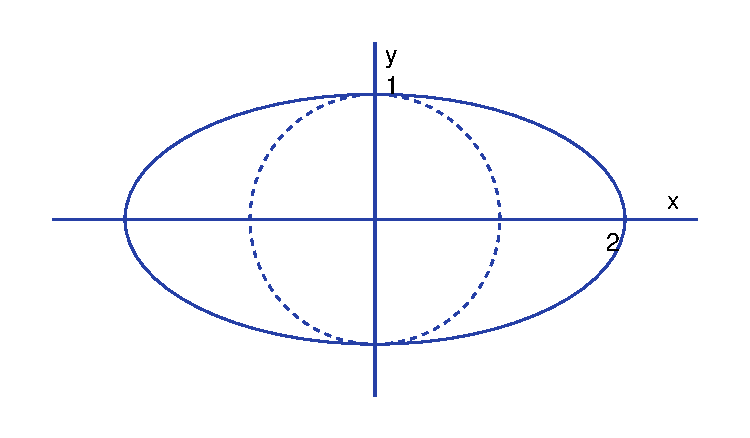
\includegraphics[width=.7\linewidth]{ellipse.pdf}
\caption{单位圆在 $A=\operatorname{diag}(2,1)$ 下的像。}\label{fig:ellipse}
\end{figure}
\begin{center}\begin{tabular}{ccc}\toprule
$x$ & $Ax$ & $\|Ax\|_2$\\\midrule
$(1,0)$ & $(2,0)$ & $2$\\
$(0,1)$ & $(0,1)$ & $1$\\\bottomrule
\end{tabular}\end{center}
\begin{exercise}\label{ex:diagonal}
设 $A=\operatorname{diag}(2,1)$。求最小的 $K\geq0$，使得对于每个 $x\in\R^2$ 都有 $\|Ax\|_2\leq K\|x\|_2$。将答案与~\eqref{eq:bound}中的 $C$ 比较。
\end{exercise}

\newpage
% SOURCE_PDF_PAGE: 4
\section{回顾与参考文献}
量词的顺序至关重要：同一个常数 $C$ 对所有向量 $x$ 都有效。该结论不要求 $A$ 可逆，也未断言 $C$ 是最优的。
\begin{enumerate}
\item 辨认~\eqref{eq:product}中的变量与下标。
\item 解释为什么在证明中取平方根能够保持不等式。
\item 核对图~\ref{fig:ellipse}与表格是否一致。
\end{enumerate}
本篇独立讲义的来源见~\cite{localnote}。参考文献标明本地原稿；这里给出的证明不需要引用外部数学文献。
\printbibliography[title={参考文献}]

\end{document}
